% Figure 2 — multi-scale linear-attention encoder and the exchange submodule.
% Standalone: pdflatex fig_arch_tikz.tex -> fig_arch_tikz.pdf; the paper can
% then \includegraphics it, or \input this file (both EM-safe, it sits in paper/).
%
% txfonts is what elsarticle's `times` option loads, so the figure's text and
% math come from the same fonts as the body -- not a lookalike.
\documentclass[border=2pt]{standalone}
\usepackage[T1]{fontenc}
\usepackage{txfonts}
\usepackage{tikz}
\usetikzlibrary{positioning, arrows.meta, calc}

% restrained palette: cool slate ground, muted brass for the two aggregation
% units, one deep ink for type and strokes.  No primaries.
% Three muted families, each carrying meaning rather than decoration:
%   sand  = the data path (capacity window in, readout out)
%   slate = the encoder (patch embedding, layer 1, layer 2 by depth)
%   brass = the two aggregation units (fuse, single-query attention)
% Three branch families, so a colour identifies a branch rather than
% decorating it: fine = teal, coarse = amber, medium = violet. Within a
% branch the tone deepens with depth (scale/embed -> layer 1 -> layer 2).
\definecolor{fink}{HTML}{2B3A45}
\definecolor{datF}{HTML}{F2EFEA}
\definecolor{datL}{HTML}{7A6F5F}
\definecolor{veilF}{HTML}{FBFAF8}
\definecolor{gridF}{HTML}{E8EBEE}
\definecolor{teal1}{HTML}{E4F0EC}
\definecolor{teal2}{HTML}{CBDFD9}
\definecolor{teal3}{HTML}{B2D0C8}
\definecolor{tealL}{HTML}{3E7268}
\definecolor{amb1}{HTML}{F4EAD4}
\definecolor{amb2}{HTML}{E8D6B4}
\definecolor{amb3}{HTML}{DCC293}
\definecolor{ambL}{HTML}{855F2C}
\definecolor{vio1}{HTML}{E9E5F3}
\definecolor{vio2}{HTML}{D5CDE7}
\definecolor{vio3}{HTML}{C0B5D9}
\definecolor{vioL}{HTML}{5C5178}

\tikzset{
  dat/.style = {draw=datL, fill=datF, rounded corners=1pt, align=center,
                font=\footnotesize, inner sep=2.2pt, minimum height=6mm},
  fine1/.style = {draw=tealL, fill=teal1, rounded corners=1pt, align=center,
                 font=\footnotesize, inner sep=2.2pt, minimum height=6mm},
  fine2/.style = {draw=tealL, fill=teal2, rounded corners=1pt, align=center,
                 font=\footnotesize, inner sep=2.2pt, minimum height=9mm},
  fine3/.style = {draw=tealL, fill=teal3, rounded corners=1pt, align=center,
                 font=\footnotesize, inner sep=2.2pt, minimum height=9mm},
  coa1/.style = {draw=ambL, fill=amb1, rounded corners=1pt, align=center,
                 font=\footnotesize, inner sep=2.2pt, minimum height=6mm},
  coa2/.style = {draw=ambL, fill=amb2, rounded corners=1pt, align=center,
                 font=\footnotesize, inner sep=2.2pt, minimum height=9mm},
  coa3/.style = {draw=ambL, fill=amb3, rounded corners=1pt, align=center,
                 font=\footnotesize, inner sep=2.2pt, minimum height=9mm},
  med1/.style = {draw=vioL, fill=vio1, rounded corners=1pt, align=center,
                 font=\footnotesize, inner sep=2.2pt, minimum height=6mm},
  med2/.style = {draw=vioL, fill=vio2, rounded corners=1pt, align=center,
                 font=\footnotesize, inner sep=2.2pt, minimum height=9mm},
  med3/.style = {draw=vioL, fill=vio3, rounded corners=1pt, align=center,
                 font=\footnotesize, inner sep=2.2pt, minimum height=9mm},
  hub/.style  = {draw=brassL, fill=brassF, circle, inner sep=1pt, font=\footnotesize},
  att/.style  = {draw=brassL, fill=brassF, rounded corners=2pt, align=center,
                font=\scriptsize, inner sep=1.5pt},
  proj/.style = {draw=brassL, fill=brassF, rounded corners=1pt, align=center,
                font=\footnotesize, inner sep=2.2pt, minimum height=6mm},
  vec/.style  = {draw=fink!45, fill=veilF, inner sep=1pt},
  tiny/.style = {font=\footnotesize, text=fink!88},
  arr/.style  = {->, >={Stealth[length=1.6mm]}, semithick, fink!80},
  bus/.style  = {semithick, fink!80},
  exh/.style  = {<->, >={Stealth[length=1.4mm]}, semithick, ambL!85},
  frame/.style= {draw=fink!30, thin},
}
\definecolor{brassF}{HTML}{EFDCC6}
\definecolor{brassL}{HTML}{8B6636}

\newcommand{\stategrid}[3]{%
  % #1 x, #2 y, #3 cell size — 4x4 grid whose lower-left corner is (#1,#2)
  \foreach \i in {0,...,3} {%
    \foreach \j in {0,...,3} {%
      \draw[very thin, fink!35, fill=gridF]
        (#1+\i*#3,#2+\j*#3) rectangle ++(#3,#3);}}}

\begin{document}
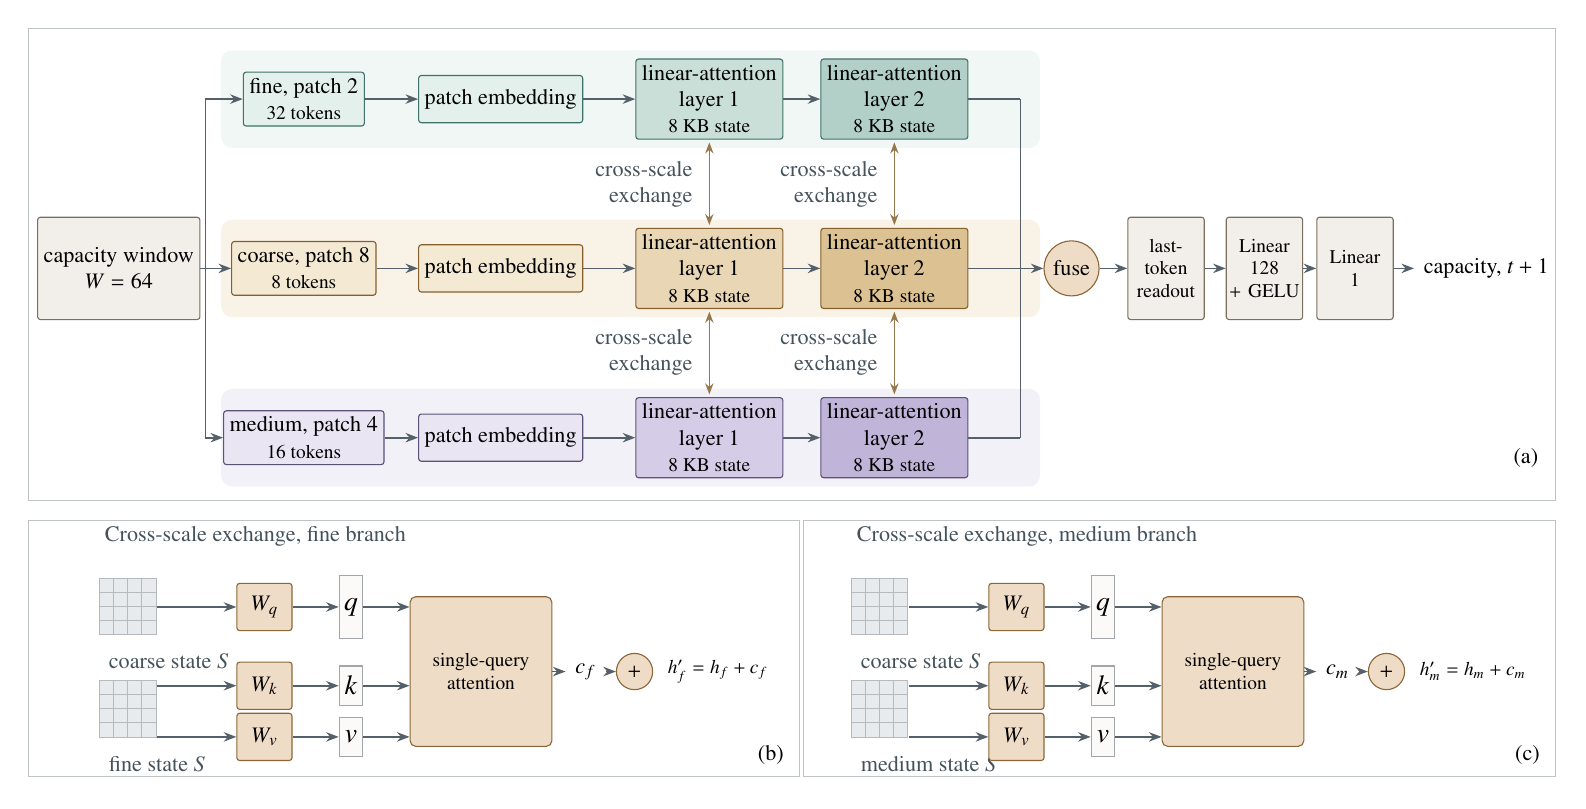
\begin{tikzpicture}

% ===================================================================== (a)
\def\yA{2.15} \def\yB{0} \def\yC{-2.15}
\def\busL{2.10} \def\busR{12.45}

% swim lanes: a faint wash behind each branch, so the three paths read
% as lanes without turning the plate into a banner
\foreach \laneY/\laneC in {2.15/teal1, 0/amb1, -2.15/vio1}{
  \fill[\laneC!55, rounded corners=4pt]
    (2.30,\laneY-0.62) rectangle (12.70,\laneY+0.62);
}

\node[dat, minimum height=13mm] (win) at (1.00,0) {capacity window\\$W=64$};
\node[hub, minimum size=7mm] (fuse) at (13.10,0) {fuse};

\node[fine1] (sA) at (3.35,\yA) {fine, patch 2\\\scriptsize 32 tokens};
\node[coa1] (sB) at (3.35,\yB) {coarse, patch 8\\\scriptsize 8 tokens};
\node[med1] (sC) at (3.35,\yC) {medium, patch 4\\\scriptsize 16 tokens};

\node[fine1] (eA) at (5.85,\yA) {patch embedding};
\node[coa1] (eB) at (5.85,\yB) {patch embedding};
\node[med1] (eC) at (5.85,\yC) {patch embedding};

\node[fine2] (aA) at (8.50,\yA) {linear-attention\\layer 1\\\scriptsize 8 KB state};
\node[coa2] (aB) at (8.50,\yB) {linear-attention\\layer 1\\\scriptsize 8 KB state};
\node[med2] (aC) at (8.50,\yC) {linear-attention\\layer 1\\\scriptsize 8 KB state};
\node[fine3] (bA) at (10.85,\yA){linear-attention\\layer 2\\\scriptsize 8 KB state};
\node[coa3] (bB) at (10.85,\yB){linear-attention\\layer 2\\\scriptsize 8 KB state};
\node[med3] (bC) at (10.85,\yC){linear-attention\\layer 2\\\scriptsize 8 KB state};

% fan out from the window: one spine to the left of every block, then a stub
% with the arrowhead into each branch.  The spine itself carries no arrows.
\draw[bus] (win.east) -- (\busL,0);
\draw[bus] (\busL,\yC) -- (\busL,\yA);
\draw[arr] (\busL,\yA) -- (sA.west);
\draw[arr] (\busL,\yB) -- (sB.west);
\draw[arr] (\busL,\yC) -- (sC.west);

\foreach \r in {A,B,C}{
  \draw[arr] (s\r) -- (e\r);
  \draw[arr] (e\r) -- (a\r);
  \draw[arr] (a\r) -- (b\r);
  \draw[bus] (b\r.east) -- (\busR,\csname y\r\endcsname);
}
% gather on one spine, then a single arrowhead into the hub
\draw[bus] (\busR,\yC) -- (\busR,\yA);
\draw[arr] (\busR,0) -- (fuse.west);

% cross-scale exchange: the coarse state is the query for the other branches
\foreach \x in {8.50,10.85}{
  \draw[exh] (\x,0.55) -- (\x,1.60);
  \draw[exh] (\x,-0.55) -- (\x,-1.60);
  \node[tiny, anchor=east, align=right] at ($(\x,1.07)+(-0.09,0)$) {cross-scale\\exchange};
  \node[tiny, anchor=east, align=right] at ($(\x,-1.07)+(-0.09,0)$) {cross-scale\\exchange};
}

\node[dat, font=\scriptsize, text width=9mm, minimum height=13mm,
                        inner sep=1pt, align=center] (last) at (14.30,0) {last-token\\readout};
\node[dat, font=\scriptsize, text width=9mm, minimum height=13mm,
                        inner sep=1pt, align=center] (lin1) at (15.55,0) {Linear 128\\+ GELU};
\node[dat, font=\scriptsize, text width=9mm, minimum height=13mm,
                        inner sep=1pt, align=center] (lin2) at (16.70,0){Linear\\1};
\node[font=\footnotesize, anchor=west] (out) at (17.45,0){capacity, $t+1$};
\draw[arr] (fuse) -- (last.west);
\draw[arr] (last) -- (lin1);
\draw[arr] (lin1) -- (lin2);
\draw[arr] (lin2) -- (out.west);

\node[anchor=south east, font=\footnotesize] at (19.15,-2.65) {(a)};
\draw[frame] (-0.15,-2.95) rectangle (19.25,3.05);

% ===================================================================== (b)(c)
% Exchange submodule.  The attention unit is a rounded rectangle, not a circle,
% so the three projections enter its left edge as three clean horizontal arrows.
\newcommand{\exchange}[3]{% #1 x-origin, #2 branch name, #3 coefficient
  \begin{scope}[shift={(#1,-6.90)}]
    \node[tiny, anchor=west] at (0.05,3.50) {Cross-scale exchange, #2 branch};

    \stategrid{0.10}{2.25}{0.18}
    \node[tiny, anchor=north west] at (0.10,2.13) {coarse state $S$};
    \stategrid{0.10}{0.95}{0.18}
    \node[tiny, anchor=north west] at (0.10,0.83) {#2 state $S$};

    \node[proj, minimum width=7mm] (wq) at (2.20,2.60) {$W_q$};
    \node[proj, minimum width=7mm] (wk) at (2.20,1.60) {$W_k$};
    \node[proj, minimum width=7mm] (wv) at (2.20,0.95) {$W_v$};
    \node[vec, minimum width=3mm, minimum height=8mm] (q) at (3.30,2.60) {$q$};
    \node[vec, minimum width=3mm, minimum height=5mm] (k) at (3.30,1.60) {$k$};
    \node[vec, minimum width=3mm, minimum height=5mm] (v) at (3.30,0.95) {$v$};

    \draw[arr] (0.84,2.60) -- (wq);  \draw[arr] (wq) -- (q);
    \draw[arr] (0.84,1.60) -- (wk);  \draw[arr] (wk) -- (k);
    \draw[arr] (0.84,0.95) -- (wv);  \draw[arr] (wv) -- (v);

    \node[att, minimum width=18mm, minimum height=19mm] (att) at (4.95,1.78)
         {single-query\\attention};
    \draw[arr] (q.east) -- (att.west |- q);
    \draw[arr] (k.east) -- (att.west |- k);
    \draw[arr] (v.east) -- (att.west |- v);

    \node[font=\footnotesize] (cf) at (6.28,1.78) {$c_{#3}$};
    \draw[arr] (att.east) -- (cf);
    \node[hub, draw=brassL, fill=brassF, minimum size=4.6mm, inner sep=0pt] (plus) at (6.90,1.78) {$+$};
    \draw[arr] (cf) -- (plus);
    \node[font=\scriptsize, anchor=west] at (7.20,1.78) {$h_{#3}' = h_{#3} + c_{#3}$};
  \end{scope}}

\exchange{0.65}{fine}{f}
\exchange{10.20}{medium}{m}

\draw[frame] (-0.15,-6.45) rectangle (9.65,-3.20);
\draw[frame] ( 9.70,-6.45) rectangle (19.25,-3.20);
\node[anchor=south east, font=\footnotesize] at (9.57,-6.42) {(b)};
\node[anchor=south east, font=\footnotesize] at (19.17,-6.42) {(c)};

\end{tikzpicture}
\end{document}
